\documentclass{standalone}
\usepackage{makeidx}
\usepackage{graphicx}
\usepackage{url}
\usepackage{bookmark,hyperref}
\usepackage{ntheorem}
\usepackage{hyperref}
\usepackage{url}
\usepackage{graphicx}
\usepackage[usenames]{color}
\usepackage{enumerate}
\usepackage{pdfpages} 
\usepackage{listings}
\usepackage{lscape}
\usepackage{stmaryrd} 
\usepackage{indentfirst}
\usepackage{multirow}
\usepackage{color}
\usepackage{booktabs}
\usepackage{float}
\usepackage{longtable}
\usepackage[toc,page]{appendix}
\usepackage{amsmath}
\usepackage{amsfonts}
\usepackage{tikz}
\usepackage{enumitem}
\usetikzlibrary{arrows,positioning,shapes.geometric}
\usepackage{textcomp}
\usepackage{multirow}
\usepackage{subfigure}
\usepackage{gensymb}
\usepackage{epstopdf}
\usepackage{mathtools}
\usepackage{float}
\usepackage{sidecap}
\usepackage{textcomp}
\usepackage{pgfplots}

%%%%%%%%%%%%%%%%%%%%%%%%%%%%%

\definecolor{gray80}{gray}{0.8}
\definecolor{chartreuse(traditional)}{rgb}{0.87, 1.0, 0.0}
\definecolor{sepia}{rgb}{0.44, 0.26, 0.08}
\definecolor{turquoise}{rgb}{0.25 0.87 0.81}
\definecolor{mulberry}{rgb}{0.77 0.29 0.55}
%%%%%%%%%%%%%%%%%%%%%%%%%%%%%


\begin{document}
	\pgfplotsset{width=8cm,compat=1.8}
	
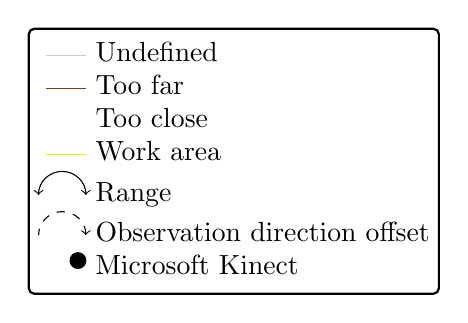
\begin{tikzpicture}
	\node[draw=black,thick,rounded corners=2pt,below left=2mm] {%
		\begin{tabular}{@{}r@{ }l@{}}
		\raisebox{2pt}{\tikz{\draw[gray80] (0,0) -- (5mm,0);}}                  & Undefined                    \\
		\raisebox{2pt}{\tikz{\draw[sepia] (0,0) -- (5mm,0);}}                   & Too far                      \\
		\raisebox{2pt}{\tikz{\draw[white] (0,0) -- (5mm,0);}}                   & Too close                    \\
		\raisebox{2pt}{\tikz{\draw[chartreuse(traditional)] (0,0) -- (5mm,0);}} & Work area                    \\
		\raisebox{2pt}{\tikz{\draw[<->, thin] (0:0) arc (0:180:0.3);}}          & Range                        \\
		\raisebox{2pt}{\tikz{\draw[<-, thin, dashed] (0:0) arc (0:180:0.3);}}   & Observation direction offset \\
		\raisebox{2pt}{\tikz{\draw[fill=black] (0, 0) circle (0.1);}}           & Microsoft Kinect             
		\end{tabular}};	
\end{tikzpicture}
\end{document}